\documentclass[11pt, letterpaper]{article}

\title{Assignment1: Questions 1 - 3}
\author{Stuart Mashaal}
\date{Sunday, October 1, 2017}

\usepackage[utf8]{inputenc}
\usepackage[margin=0.75in]{geometry}
\usepackage{graphicx}
\usepackage{indentfirst}
\usepackage{amsmath}

\begin{document}
\maketitle

\section*{Question 1}

Uniprogramming is a computing paradigm wherein the computer can only manage and run a single process at once.  This means that if there are three process to run and each one performs a large IO operation, the computer will run them each separately and sequentially with the CPU idle during each of the large IO operations.

\begin{center}
    
\includegraphics[width=0.5\textwidth]{uniprogramming.png}
\end{center}

Multiprogramming is a computing paradigm wherein the computer can manage multiple processes at once, whether or not it can actually execute the instructions of multiple processes in parallel.  This means that if there are three processes to run and each one performs a large IO operation, a single-core CPU would not idle during the large IO operations.  Instead, while the first process is waiting for IO, it will run another process and while the second process is waiting on IO it will run another (and so on, as necessary).

\begin{center}
    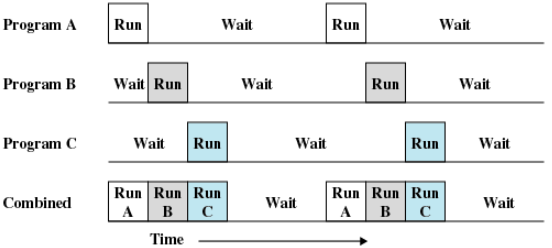
\includegraphics[width=0.5\textwidth]{multiprogramming.png}
\end{center}

Time-sharing is the ability of a computer system to accommodate multiple users simultanneously.  A time-sharing system is one that uses multiprogramming to allow multiple users to interact with the system at the same time.  While all but one of the users is idle, the system can record (for example) the key-presses of one user.  Time-sharing systems are really just multiprogramming systems in which one of the processes that the system is constantly switching between is the reading in of multiple users' input.


\newpage

\section*{Question 2}

As stated in my answer to Question 1, a uniprogramming system is a system that can only run and manage a single process at once.  So, once a job starts, no matter how many parts of that job don't even use the CPU, the CPU will not execute the instructions of any other job.  This means that jobs A, B, and C will run one after the other.  Therefore, the time taken to finish the three jobs on a uniprogramming system is given by $$3 \cdot (2\text{ms} + 10\text{ms} + 4\text{ms}) = 48\text{ms}$$

\end{document}
